\chapter{Dissemination of culture}
\taskID{30}{Axelrod's model for dissemination of culture}
\label{ch:culture}

\section{Social influence and consensus formation}
The \emph{Axelrod's model} aims at understanding the formation of cultural domains and the effects of a convergent social influence, describing how local convergence can generate global polarization. Here, the term \emph{culture} refers to the set of individual attributes shaped by social dynamics. The following mechanism is based on three principles: an agent-based approach, the lack of a central authority, and adaptive - rather than rational - behavior \cite{axelrod1997dissemination}. \\
The model is defined on top of a network where each node $i$ has a set of $F$ integer variables $\sigma_{i, F}$ representing the cultural "features". Each feature $f$ is initially drawn randomly from a Poisson distribution of parameter $q$. Thus, $q$ measures the initial cultural variability. At each time step, a pair of nearest neighbors $(i, j)$ and a feature $f$ are randomly selected. If $\sigma_{i, f} \neq \sigma_{j, f}$ nothing happens. If instead $\sigma_{i, f} = \sigma_{j, f}$ then nodes $i$ and $j$ interact and another feature $g$ such that $\sigma_{i, g} \neq \sigma_{j, g}$ is chosen and set equal: $\sigma_{i, g} \to \sigma_{i, g} = \sigma_{j, g}$. \\
Note that a link is \emph{active} if the number of shared features is strictly greater than zero and lower than $F$ and the total diversity (namely the number of different values of $f$ in the system) always decreases. The dynamics converge to one of the many \emph{absorbing states} such that, on each link, either all features are equal or they are all different \cite{castellano2000nonequilibrium, miguel2005binary}. 

\begin{figure}[h]
    \centering
    \begin{minipage}{0.25\textwidth}
        \centering
        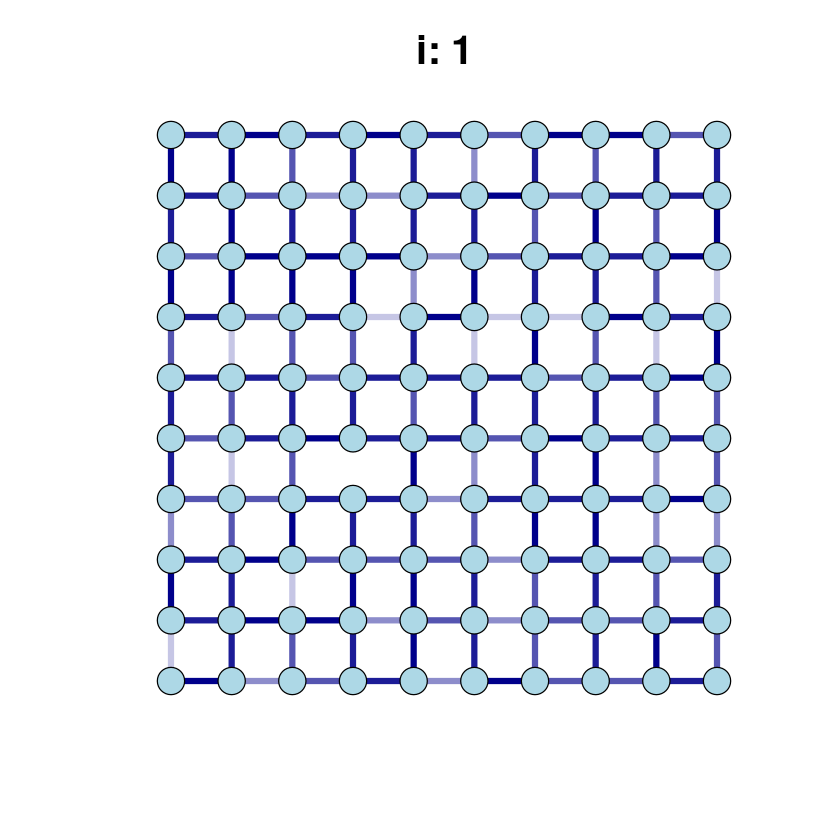
\includegraphics[width=\textwidth]{images/task30/dyn1.png}
    \end{minipage}\hfill
    \begin{minipage}{0.25\textwidth}
        \centering
        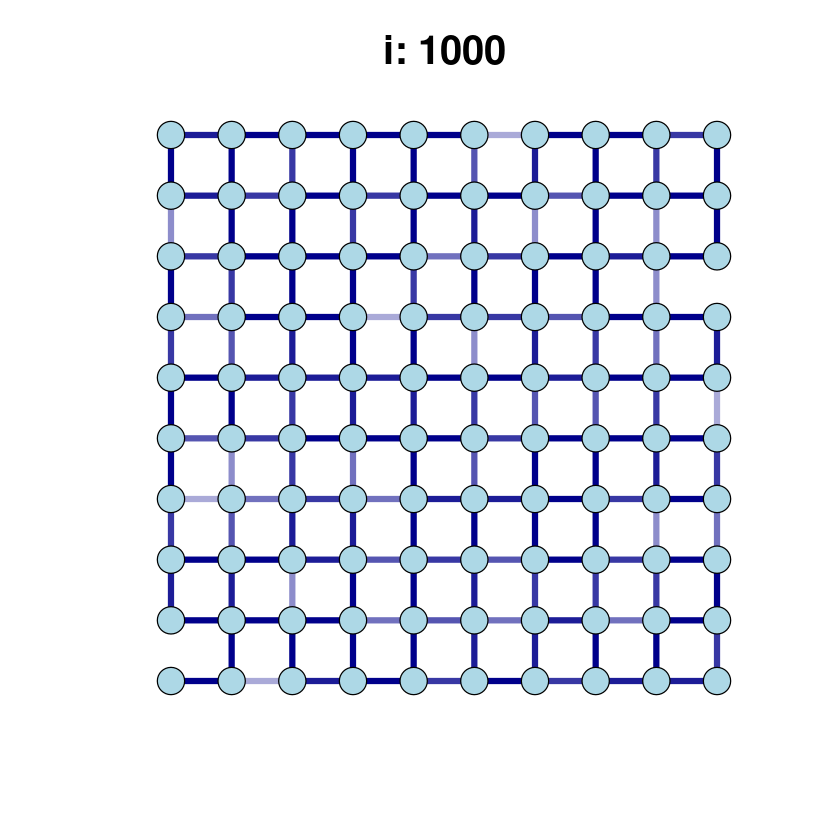
\includegraphics[width=\textwidth]{images/task30/dyn2.png}
    \end{minipage}\hfill
    \begin{minipage}{0.25\textwidth}
        \centering
        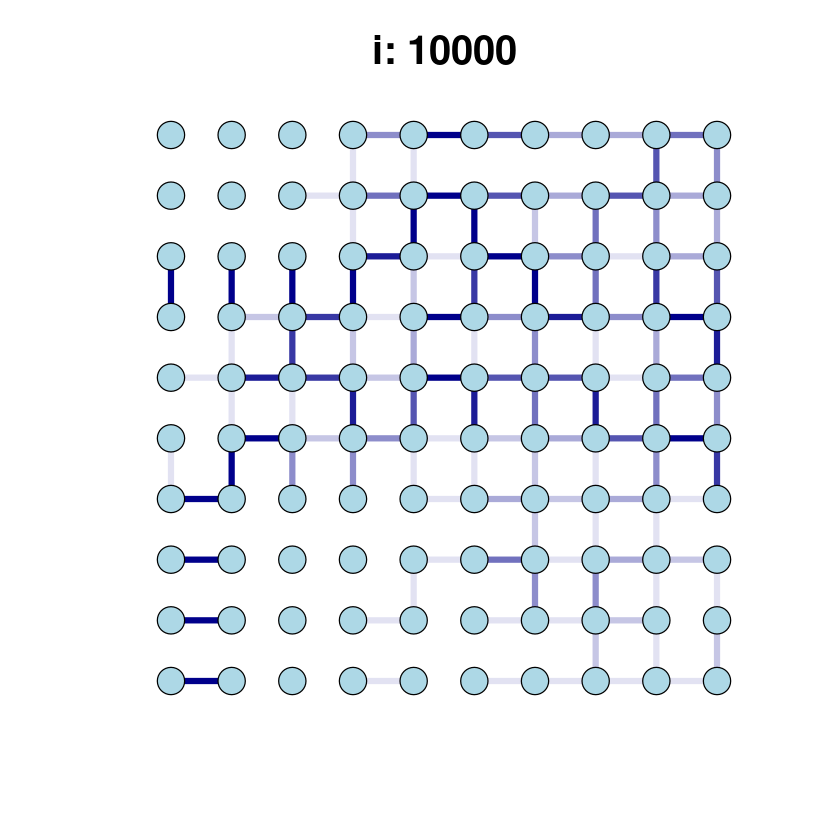
\includegraphics[width=\textwidth]{images/task30/dyn3.png}
    \end{minipage}\hfill
    \begin{minipage}{0.25\textwidth}
        \centering
        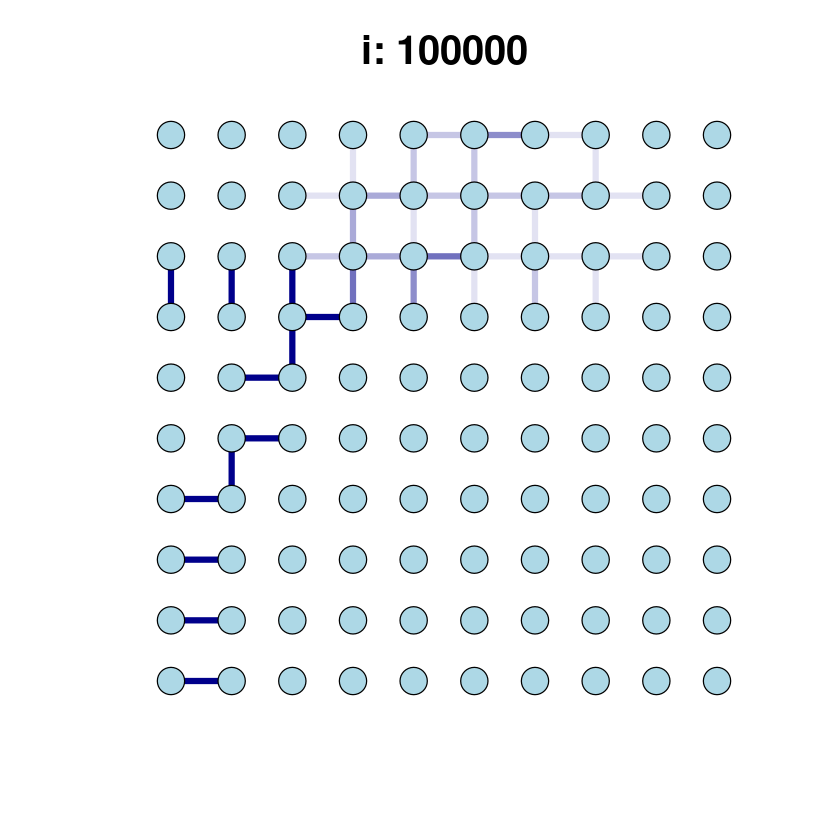
\includegraphics[width=\textwidth]{images/task30/dyn4.png}
    \end{minipage}
    \vspace{-0.5cm}
    \caption{Example of consensus formation: the darker the blue at the edge, the fewer features the nodes share. Four snapshots of the dynamics simulated on top of a $2$d regular lattice of size $L=10$. Here, $F=10$ and $q=4$.}
    \label{fig:figures}
\end{figure}

\noindent An interesting particularity of this model is the existence of a phase transition between a "culturally polarized" and "culturally fragmented" final state. This can be studied by analyzing the size of the largest cultural domain $s_{\text{max}}$ (the order parameter) as a function of the initial variability parameter $q$ \cite{castellano2000nonequilibrium, miguel2005binary}. The transition becomes sharp and well-defined for large systems \cite{miguel2005binary}, thus I was not able to properly characterize it in this report due to the lack of proper computational resources \footnote{An attempt can be found in the supplementary material \ref{ch:sm_culture}}.

\vspace{-0.1cm}
\section{Numerical simulations}
The model has been tested in five different networks, recording both the size of the largest cultural domain $s_\text{max}$ and the density of active links $n_\text{active}$ varying $q$ and $F$. The networks are obtained via Erdős–Rényi ($p=2\times10^{-3}$, $7\times10^{-3}$, $1.2\times10^{-2}$) and Barabasi-Albert ($m=1$, $5$) instances. Each network has $N=2\times10^3$ nodes and the results refer to $4$ independent simulations of $5\times10^7$ iterations each. Moreover, $3$ massive simulations have been done in $50\times 50$ regular lattices for $10^{10}$ time steps. \\

\vspace{-0.1cm}
\begin{figure}[h] 
    \centering
    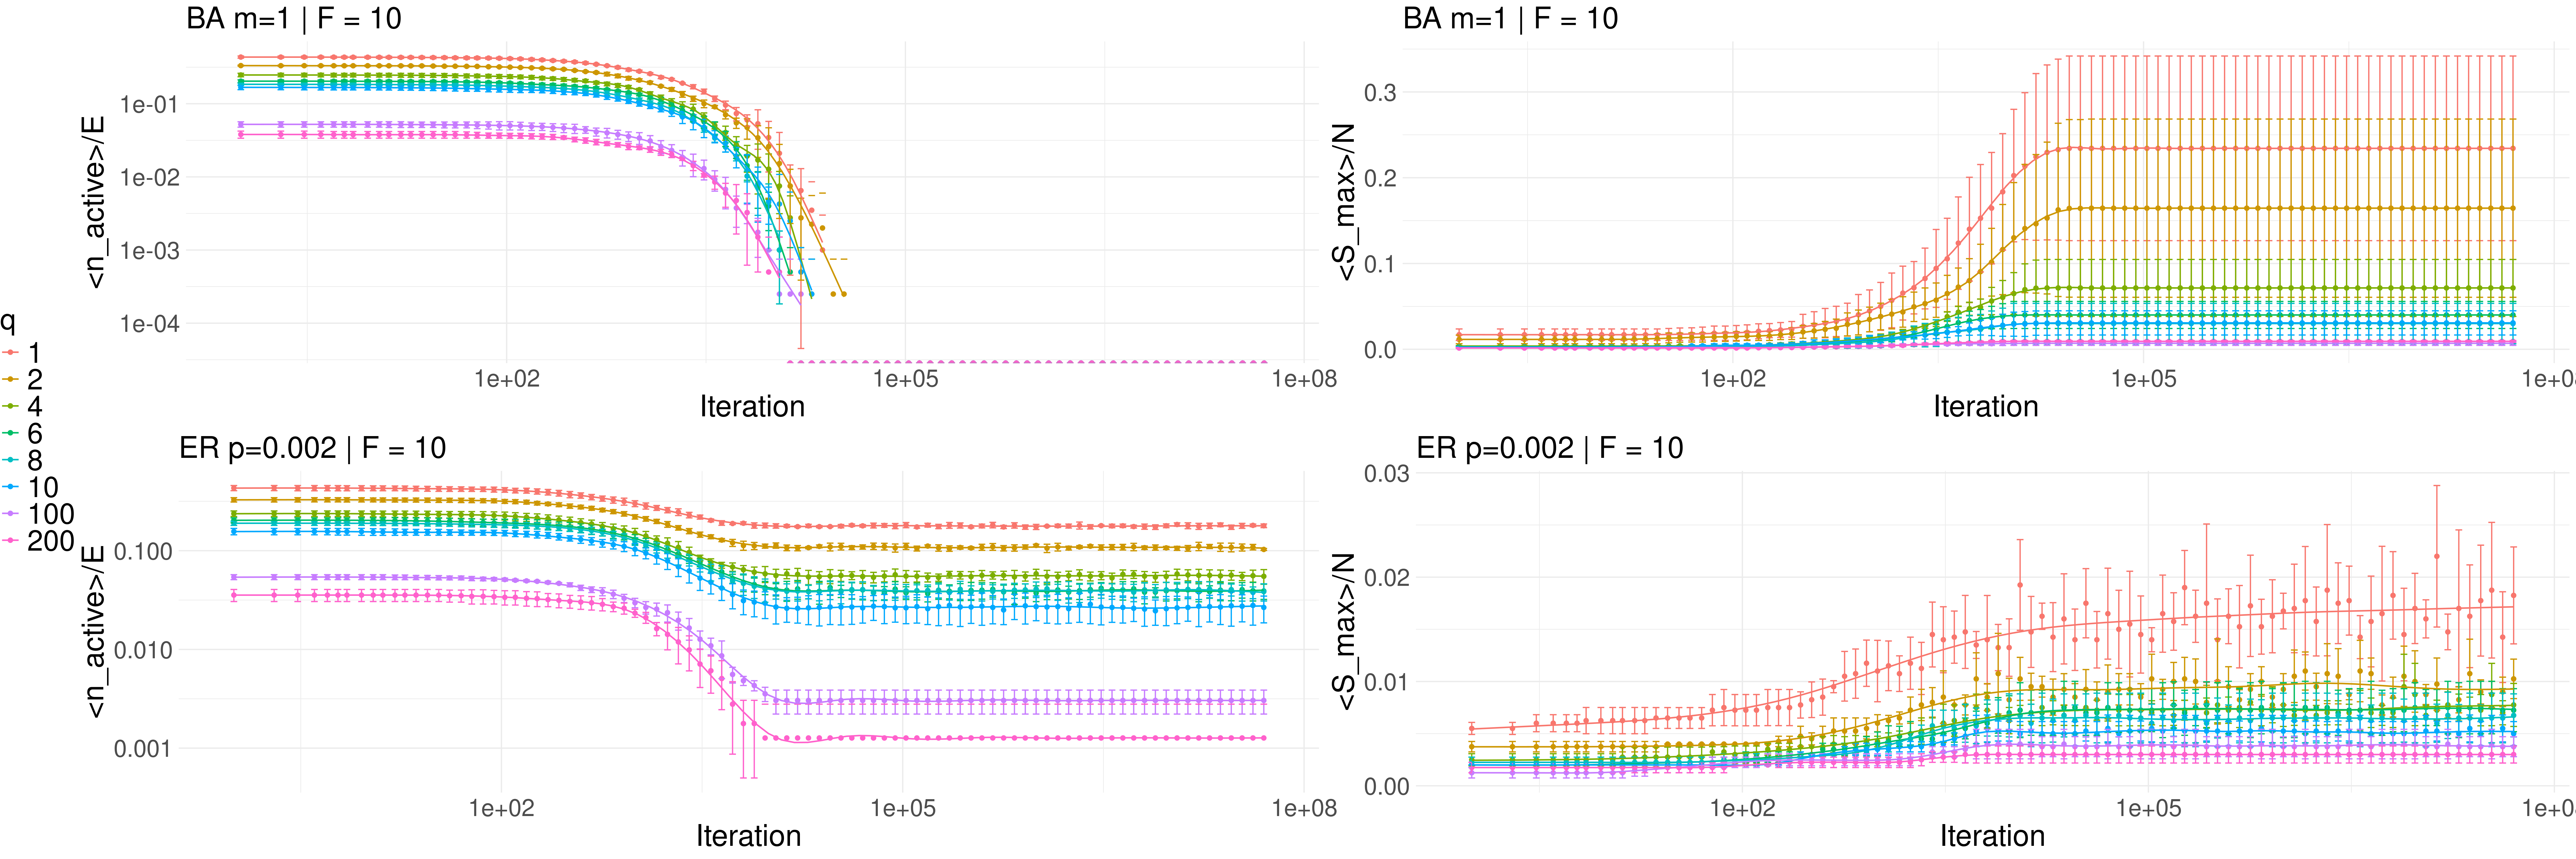
\includegraphics[width=1\textwidth]{images/task30/ba-er.png} 
    \vspace{-0.5cm}
    \caption{Evolution of the $n_\text{active}$ (left) and  $s_\text{max}$ (right) in BA $m=1$ (top) and ER $p=0.002$ (bottom) networks. $F=10$.}
    \label{fig:culture1} 
\end{figure}

\vspace{-0.1cm}
\noindent Figure \ref{fig:culture1} and \ref{fig:culture2} make evident the role of the network topology in the final state, even for compatible values of the average degree. The dynamics on top of BA networks converge faster to a frozen state both in the case of global consensus (low values of $q$) and cultural fragmentation. Other figures can be found in the supplementary material \ref{ch:sm_culture}. The natural continuation of this analysis is to increase the number of nodes and the number of iterations. 

\begin{figure}[h] 
    \centering
    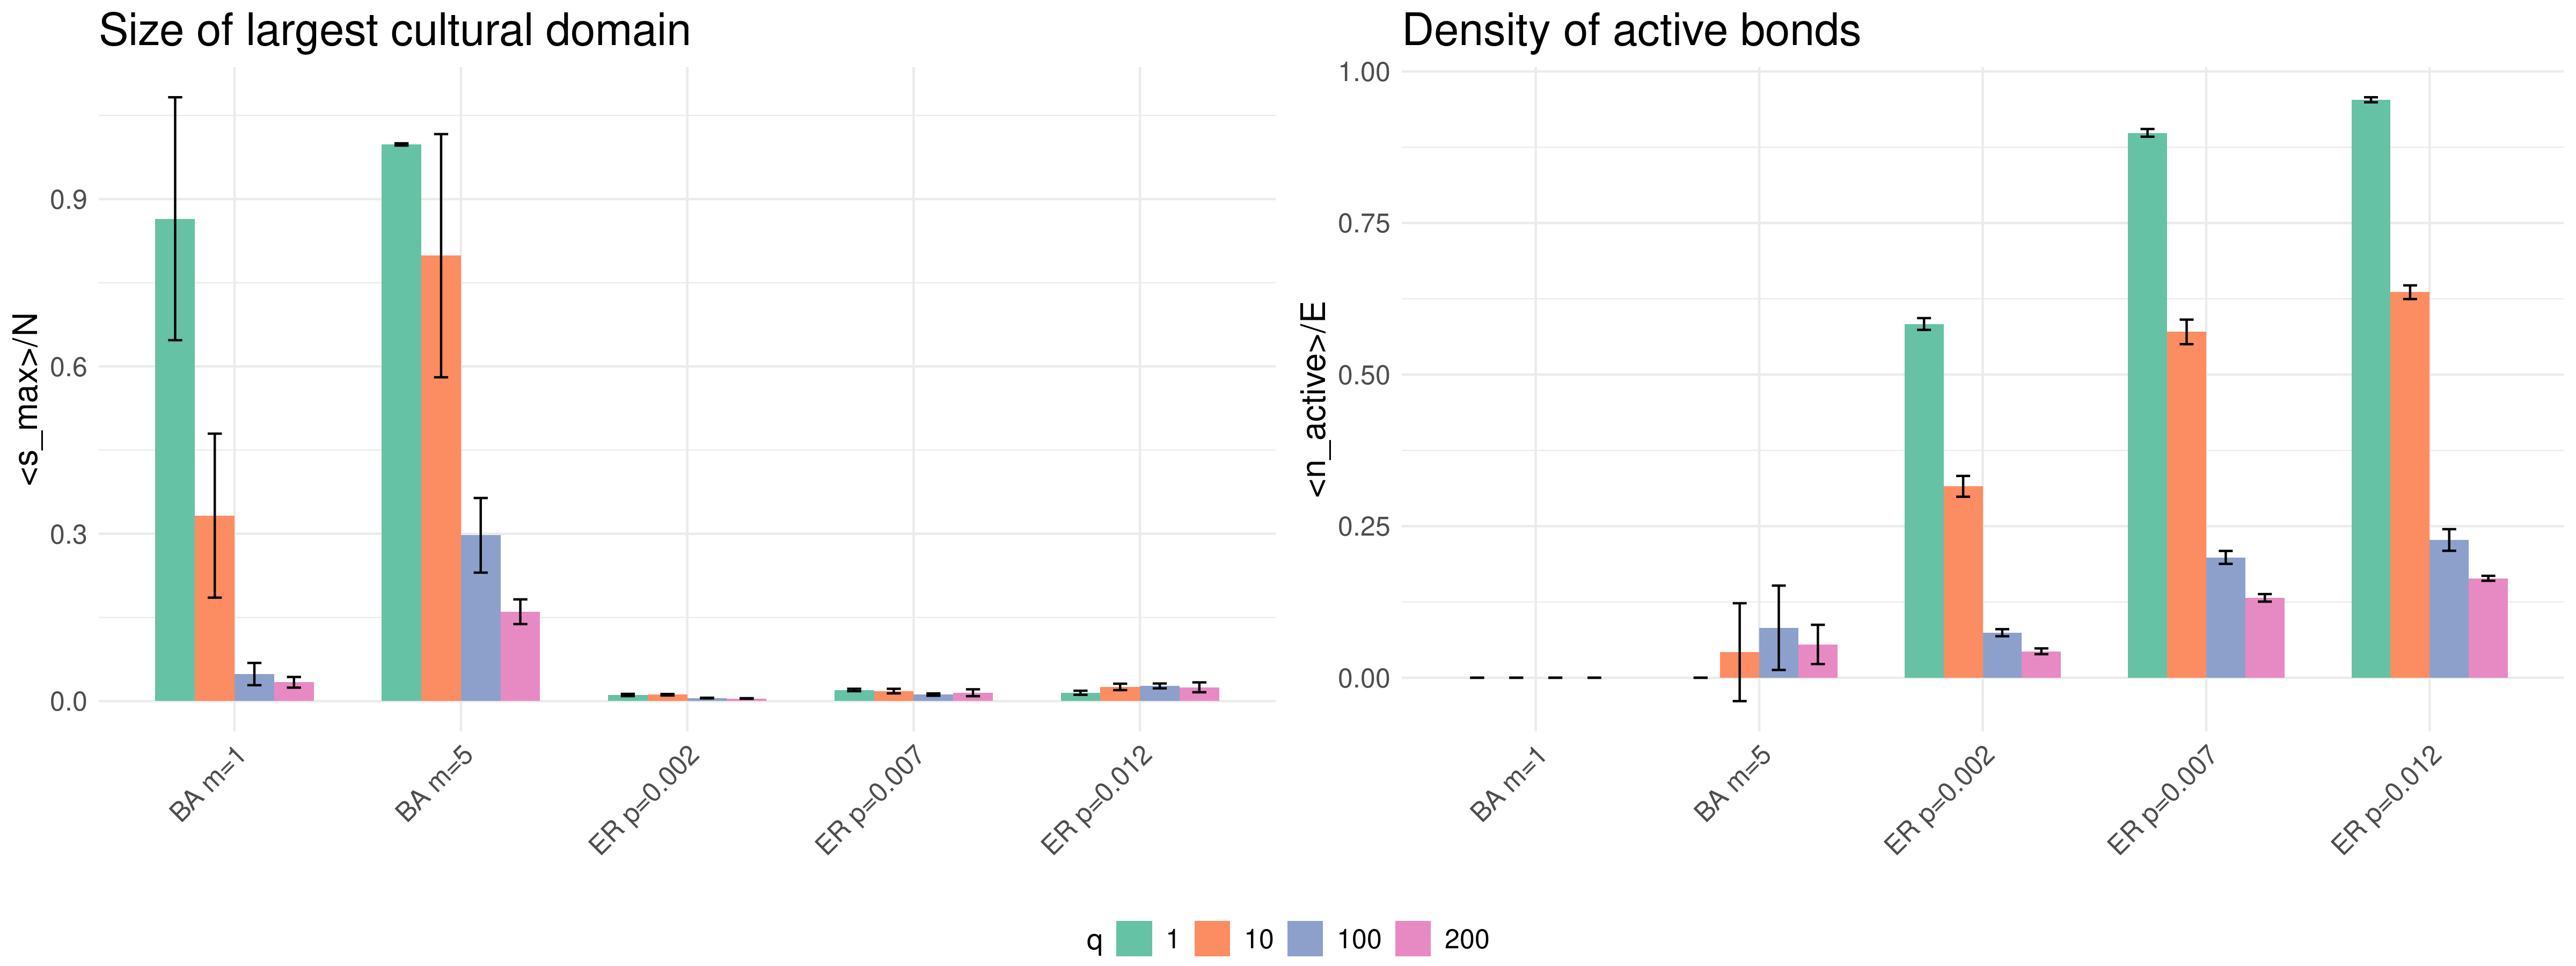
\includegraphics[width=1\textwidth]{images/task30/culturalconvergence.png} 
    \vspace{-0.5cm}
    \caption{$s_\text{max}$ and $n_\text{active}$ after $5 \times 10^7$ time steps. $N=10^3$, $F=10$.}
    \label{fig:culture2} 
\end{figure}